\chapter{Clustering}
In questo capitolo mostreremo il comportamento 
degli algoritmi di clustering KMeans, DBSCAN 
e Hierarchical applicati al nostro insieme di 
dati.

Il dataset utile per questa fase \`e stato
ottenuto eliminando gli attributi categorici
\texttt{education, sex} e \texttt{status} 
e l'attributo \texttt{credit\_default} 
poich\`e il clustering rientra tra 
gli addestramenti di tipo non supervisionato.

\section{KMeans}

Il miglior parametro \textit{k} con cui eseguire 
KMeans \`e stato stimato calcolando la 
\textit{SSE} variando \textit{k} su un range da 
2 a 20, con metrica di distanza euclidea. 
In figura~\ref{fig:best_k} sono riportati 
i risultati ottenuti. Si nota che il cambio di
pendenza della curva si trova quando \textit{k}
vale 7. A partire da ci\`o abbiamo eseguito l'algoritmo
per $k\in[3,10]$, reiterando per ogni passo 50 volte
KMeans per evitare che la scelta casuale dei centroidi
influenzasse i risultati e calcolando in questo caso
anche l'indice di Silhouette per i cluster trovati.
In seguito a queste analisi abbiamo constatato come
i cluster ottenuti per $k=4$ siano i pi\`u significativi,
la nostra considerazione \`e stata rafforzata dal fatto
che il clustering ottenuto per $k=4$ presenta il valore
dell'indice di \sil pi\`u alto trovato.

\begin{figure}[H]
	\centering
	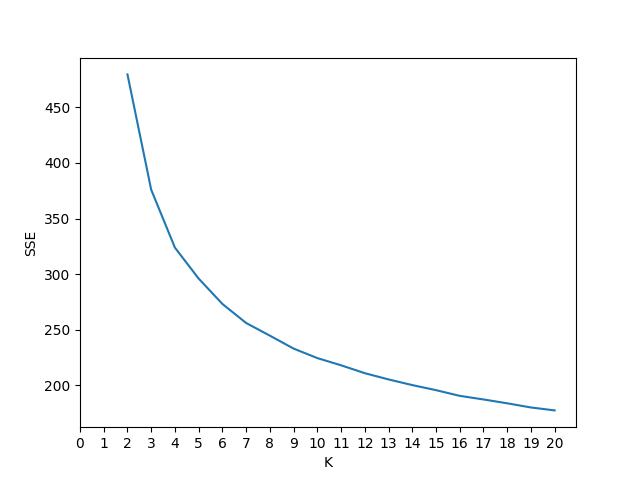
\includegraphics[width=10cm]{img/best_k.png}
	\caption[LOF entry]{SSE}
	\label{fig:best_k}
\end{figure} 

Di seguito analizziamo i cluster trovati, assegnando loro 
un nome che contraddistingua le caratteristiche 
di ogni cluster.

\paragraph{Senza rischio}
Cluster costituito da 3032 persone. Pagano in modo puntuale
le loro spese ogni mese senza registrare ritardi e compiono 
solitamente spese di bassa entit\`a. Non costituiscono alcuna
minaccia per la banca.

\paragraph{Piccoli pagatori}
Gruppo di 4832 persone. Sono soliti fare un uso abbastanza 
intensivo del revolving credit per pagare le loro spese. 
Anch'essi registrano spese di bassa entit\`a e non commettono
gravi ritardi nel pagamento, per questo motivo rientrano tra
clienti credibili per la banca.

\paragraph{Grandi pagatori}
Cluster di 1083 persone. Come per i \textit{piccoli pagatori}, 
anch'essi sono soliti usare la modalit\`a di pagamento 
rateizzata anche se le loro spese sono generalmente molto elevate.
Non si registrano comunque grossi ritardi ed \'e per questo che
rientrano comunque tra il gruppo di clienti credibili.

\paragraph{Ritardatari}
Gruppo formato da 1053 persone. Registrano spese di media entit\`a
ma al contrario degli altri tre gruppi si verificano gravi ritardi
nei pagamenti. Sono il cluster di persone che, infine, finisce in
credit default e non sono clienti credibili per la banca.

In figura~\ref{fig:centers} si sono plottate una selezione
delle coordinate dei centroidi, mostrando chiaramente dove i quattro
cluster trovati differiscono maggiormente.

\begin{figure}[H]
	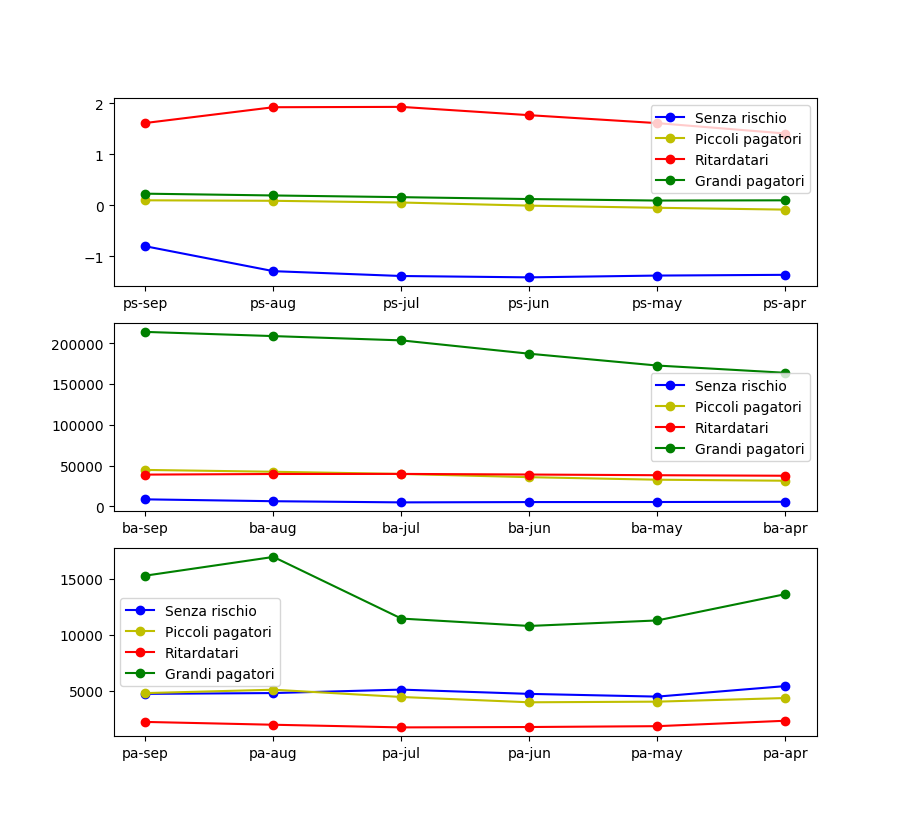
\includegraphics[width=\linewidth]{img/centers_kmeans.png}
	\caption{Caratteristiche dei cluster}
	\label{fig:centers}
\end{figure} 

\begin{figure}[H]
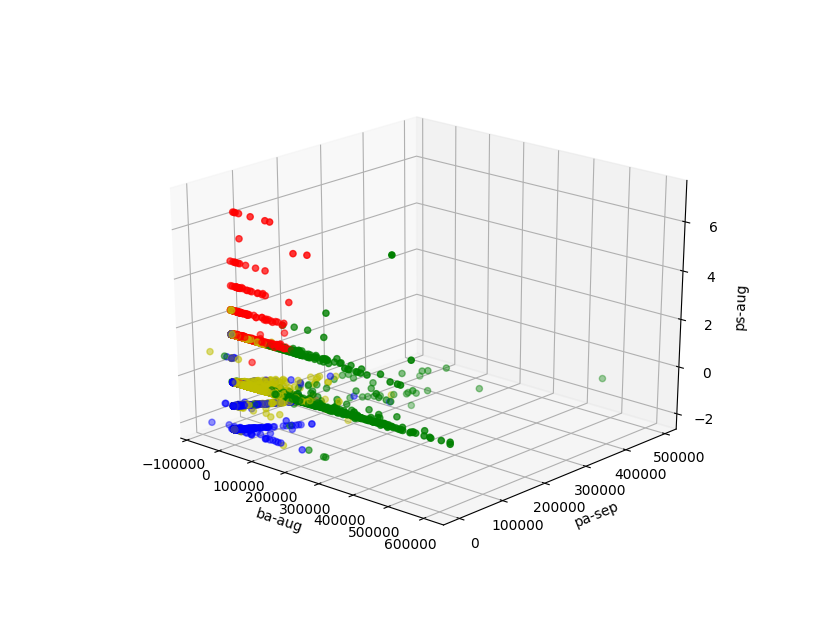
\includegraphics[width=\linewidth]{img/kmeans.png}
\caption{Distribuzione dei cluster su un pagamento mensile}
\label{fig:kmeans}
\end{figure} 

Infine si \`e plottato su un un grafico 3D (figura~\ref{fig:kmeans}
la distribuzione dei cluster su un pagamento mensile (in questo 
caso si e' preso il pagamento del mese di agosto) ed abbiamo 
notato che la distribuzione \`e rispettata per ogni terna di attributi
validi costruibili sull'insieme dei mesi disponibili.
In particolare il cluster dei \textit{ritardari} si posiziona sempre
a valori molto elevati di \texttt{payment status}, mentre vale
esattamente il contrario per il cluster dei \textit{senza rischio}.
Le tre
dimensioni scelte per l'esempio sono \texttt{billing amount august},
\texttt{payment status august} e \texttt{payment amount september}.

Infine riportiamo una tabella contenente la media e la deviazione 
standard di ogni cluster individuato. Per ragioni di spazio per 
gli attributi \texttt{payment status}, \texttt{payment amount}
e \texttt{billing amount} mostriamo i valori degli ultimi due mesi.

\begin{center}
	
\begin{tabular}{c|c|c|c|c|c|c}
	\hline
	\textbf{Cluster} & \textbf{ps-sep} 
	& \textbf{ps-aug} & \textbf{pa-sep} 
	& \textbf{pa-aug}\\
	\hline
	Senza rischio & 
	$-0.8 (\pm 1.0)$ & 
	$-1.3 (\pm 0.7)$ &
	$4.7k (\pm 12.0k)$ &
	$4.8k (\pm 14.3)$\\
	\hline
	Piccoli pagatori & 
	$0.09 (\pm 0.71)$ & 
	$0.08 (\pm 0.71)$ &
	$4.8k (\pm 10k)$ &
	$5k (\pm 13.3k)$\\
	\hline
	Grandi pagatori & 
	$0.22 (\pm 0.75)$ & 
	$0.19 (\pm 0.71)$ &
	$15k (\pm 35k)$ &
	$16k (\pm 56k)$\\
	\hline
	Ritardatari & 
	$1.60 (\pm 1.18)$ & 
	$1.90 (\pm 1.03)$ &
	$2k (\pm 3.4k)$ &
	$1.8k (\pm 3.0k)$\\
	\hline
	& 
	\textbf{ba-sep} & 
	\textbf{ba-aug} & 
	\textbf{limit} & 
	\textbf{age} &\\
	\hline
	Senza rischio & 
	$8.7k (\pm 21k)$ &
	$6.4k (\pm 16k)$ &
	$215k (\pm 126k)$ &
	$36 (\pm 8)$\\
	\hline
	Piccoli pagatori &
	$44k (\pm 39k)$ &
	$42k (\pm 35k)$ &
	$130k (\pm 113k)$ &
	$35 (\pm 9)$\\
	\hline
	Grandi pagatori &
	$213k (\pm 93k)$ &
	$208k (\pm 88k)$ &
	$281k (\pm 115k)$ &
	$37 (\pm 8)$\\
	\hline
	Ritardatari &
	$38k (\pm 35k)$ &
	$39k (\pm 36k)$ &
	$79k (\pm 68k)$ &
	$34 (\pm 8)$\\
	\hline
	& 
	\textbf{sex} & 
	\textbf{status} & 
	\textbf{education} & 
	\textbf{default}\\
	\hline
	Senza rischio & 
	F &
	Single &
	University&
	17\%\\
	\hline
	Piccoli pagatori & 
	F &
	Single &
	University&
	18\%\\
	\hline
	Grandi pagatori & 
	F &
	Single &
	University&
	19\%\\
	\hline
	Ritardatari & 
	F &
	Single &
	University&
	61\%\\
	\hline
\end{tabular}

\end{center}

Si noti come il gruppo dei ritardatari ha un limite imposto dalla banca molto pi\`u basso rispetto agli altri cluster. Segno che la banca ha valutato ottimamente i profili nella scelta di concessione del credito.

\section{DBSCAN}L'algoritmo DBSCAN \`e stato eseguito su un dataset
modificato rispetto alla esecuzione del KMeans.
Questo \`e stato dovuto per permettere all'algoritmo
di funzionare al meglio. Dopo molteplici esperimenti
infatti i migliori risultati per DBSCAN sono stati ottenuti
su un dataset composto dai soli attributi 
\texttt{payment status} di ciascun mese. Ci\`o \`e in linea
con la teoria in quanto DBSCAN ha problemi su dati con un 
numero troppo elevato di dimensioni.
Per stimare i parametri ottimali dell'algoritmo si sono
utilizzati i grafici del k-dist$^2$, utilizzando la 
distanza di Manhatthan. I valori che ci hanno permesso di
ottenere un (primo) risultato soddisfacente sono stati
$\varepsilon=0.30$ e $minPoints=350$.
Il primo risultato \`e stato l'individuazione da parte
di DBSCAN di due cluster di dimensioni molto diverse tra
loro ma con un significato molto forte.

\paragraph{Senza rischio}
Composto da 8597 persone, formato da persone che non
costituiscono alcun rischio in quanto i loro valori 
di payment status sono costantemente sotto lo 0.

\paragraph{Ritardatari}
Composto da sole 454 unit\`a. Ci\`o che lo contraddistingue
\`e un costante ritardo nei pagamenti dei propri debiti.
Queste sono le persone che maggiormente rappresentano
un rischio di perdita di credito per la banca.

Data la notevole disparit\`a di dimensioni dei due cluster, 
abbiamo deciso di eseguire nuovamente DBSCAN sul cluster
dei senza rischio al fine di verificare se anch'esso avrebbe
trovato la conformazione dei tre cluster individuati da KMeans.
Abbiamo rieseguito l'algoritmo con gli stessi parametri e il
risultato \`e stato l'individuazione di tre cluster con una 
notevole quantit\`a di rumore. 

\paragraph{Rifinanziatori}
Cluster composto da 3271 persone. Sono contraddistinti da un uso 
intensivo del revolving credit. Le spese sono di entit\`a media.
Per questo motivo sospettiamo sia un merge tra i
\textit{Grandi pagatori} e \textit{Piccoli pagatori} trovati
da KMeans.

\paragraph{Senza rischio}
Cluster composto da 635 persone. Sono le persone che pagano
sempre in orario, ogni mese rispettano la scadenza e
ripagano in pieno il loro debito. Hanno caratteristiche
molto simili all'omonimo di KMeans.

\paragraph{No consumption}
Cluster composto da 703 persone. Questa \`e la novit\`a 
rispetto a KMeans. Questo cluster incorpora tutte le persone
che non fanno uso del loro credito, evidenziato da un valore
di \textit{No consumption} molto ripetuto.

In conclusione, DBSCAN in qualche modo valida i risultati
ottenuti da KMeans, in quanto due diversi algoritmi, su due
selezioni diverse del dataset hanno trovato dei risultati
molto simili, fatta eccezione per il cluster dei
\textit{No consumption}.

Di seguito riportiamo una tabella riassuntiva delle
caratteristiche dei cluster trovati:

\begin{center}
	
	\begin{tabular}{c|c|c|c|c|c|c}
		\hline
		\textbf{Cluster} & \textbf{ps-sep} 
		& \textbf{ps-aug} & \textbf{pa-sep} 
		& \textbf{pa-aug}\\
		\hline
		Senza rischio & 
		$-1.0 (\pm 0.0)$ & 
		$-1.0 (\pm 0.0)$ &
		$6.8k (\pm 14.0k)$ &
		$6.4k (\pm 12k)$\\
		\hline
		No consumption & 
		$-2.0 (\pm 0.71)$ & 
		$-2.0 (\pm 0.71)$ &
		$4.8k (\pm 14k)$ &
		$5k (\pm 14k)$\\
		\hline
		Rifinanziatori & 
		$0.0 (\pm 0.0)$ & 
		$0.0 (\pm 0.0)$ &
		$6k (\pm 13k)$ &
		$5.9k (\pm 16k)$\\
		\hline
		Ritardatari & 
		$1.72 (\pm 0.68)$ & 
		$2.10 (\pm 0.33)$ &
		$2.5k (\pm 3.9k)$ &
		$2.5k (\pm 4.3k)$\\
		\hline
		& 
		\textbf{ba-sep} & 
		\textbf{ba-aug} & 
		\textbf{limit} & 
		\textbf{age} &\\
		\hline
		Senza rischio & 
		$6.3k (\pm 12k)$ &
		$6.4k (\pm 12k)$ &
		$221k (\pm 123k)$ &
		$36 (\pm 8)$\\
		\hline
		No consumption &
		$7k (\pm 23k)$ &
		$6k (\pm 19k)$ &
		$248k (\pm 122k)$ &
		$36 (\pm 7)$\\
		\hline
		Rifinanziatori &
		$93k (\pm 88k)$ &
		$89k (\pm 85k)$ &
		$161k (\pm 128k)$ &
		$35 (\pm 9)$\\
		\hline
		Ritardatari &
		$52k (\pm 56k)$ &
		$53k (\pm 56k)$ &
		$92k (\pm 68k)$ &
		$35 (\pm 9)$\\
		\hline
		& 
		\textbf{sex} & 
		\textbf{status} & 
		\textbf{education} & 
		\textbf{default}\\
		\hline
		Senza rischio & 
		F &
		Single &
		Graduate school&
		14\%\\
		\hline
		No consumption & 
		F &
		Single &
		Graduate School &
		11\%\\
		\hline
		Rifinanziatori & 
		F &
		Single &
		University&
		9\%\\
		\hline
		Ritardatari & 
		F &
		Single &
		University&
		68\%\\
		\hline
	\end{tabular}
\end{center}


\section{Hierarchical Clustering}
Per l'algoritmo di Hierarchical Clustering si \`e utilizzato un dataset privo delle varibili categoriche \texttt{education, status, sex} e della variabile \texttt{credit\_default}, poich\`e come pi\`u volte sottolineato, l'addestramento \`e di tipo non supervisionato. Inoltre dopo una serie di test si \`e deciso di eliminare anche la variabile \texttt{age}, senza la quale si sono raggiunti buoni risultati. Per parametri del clustering gerarchico si \`e scelta la \textbf{formula euclidea} per la distanza dato che l'utilizzo delle metriche \textit{supremum e manhattan} ha portato alla generazione di clusters di cardinalità troppo diverse. Per lo stesso motivo si \`e scelto come metodo aggregativo il \textbf{Metodo di Ward}, o della devianza minima, attraverso il quale si \`e raggiunto il miglior risultato in termini di ordine di grandezza delle dimensioni dei cluster. Gli altri metodi utilizzati $($single, complete, average$)$ non hanno portato a risultati accettabili.
\begin{figure}[H]
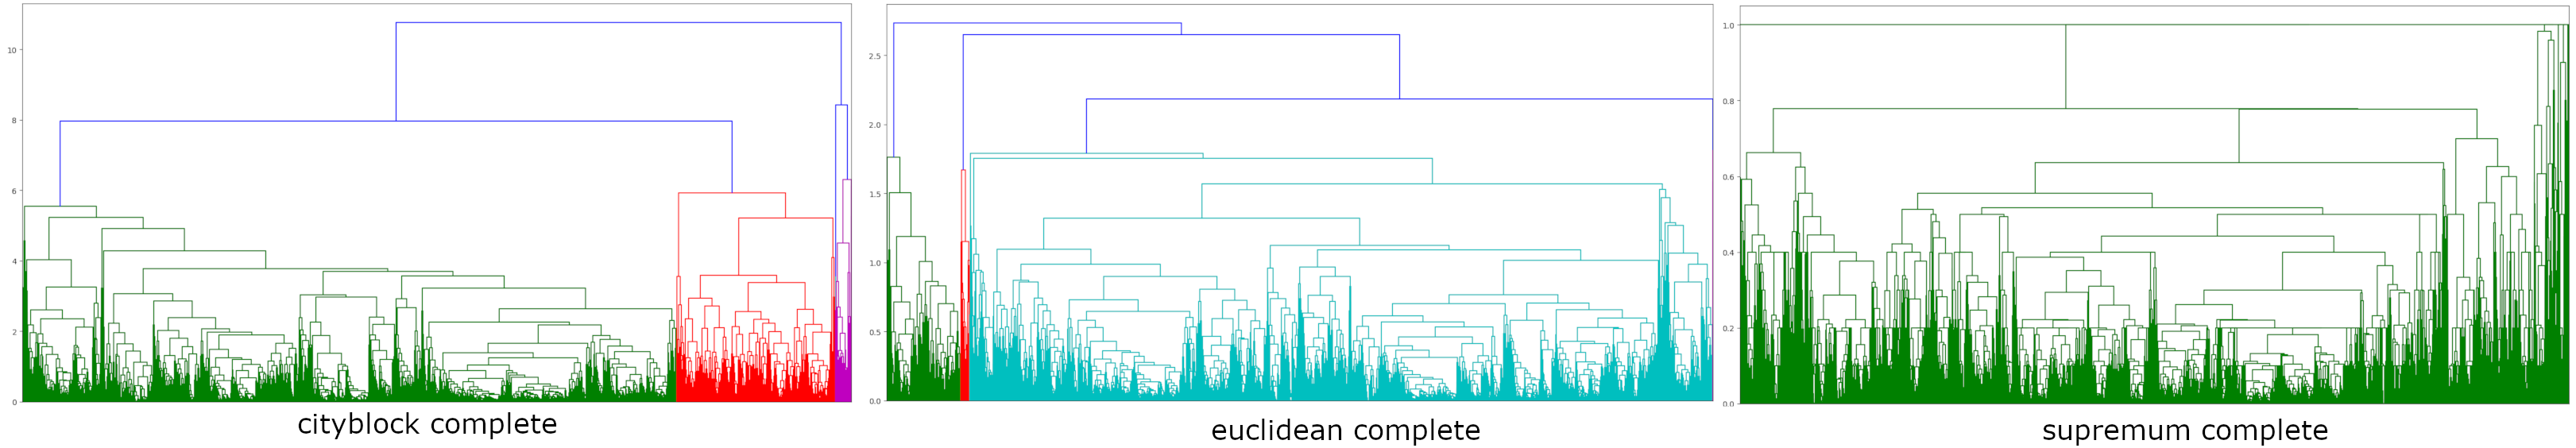
\includegraphics[width=\linewidth]{img/complete.png}
\caption{Esempio di dendrogrammi ricavati durante il test. I 3 casi in figura non sono stati considerati cluster accettabili.}
\label{dendro-complete}
\end{figure} 
\mbox{}\\
\mbox{}\\
Utilizzando la metrica euclidea e il metodo di Ward per il merging, si \`e deciso di settare la soglia a 15.2 ottenendo 4 cluster di dimensioni comparabili. In figura~\ref{euward} sono visualizzabili i clusters ottenuti mentre in figura ~\ref{euwardtrunc} \`e stato effettuato raggruppamento dei non singleton pi\`u profondi e sono stati aggiunti dei label per effettuare il troncamento a 15.2.
\begin{figure}[!htb]
\minipage{0.48\textwidth}
  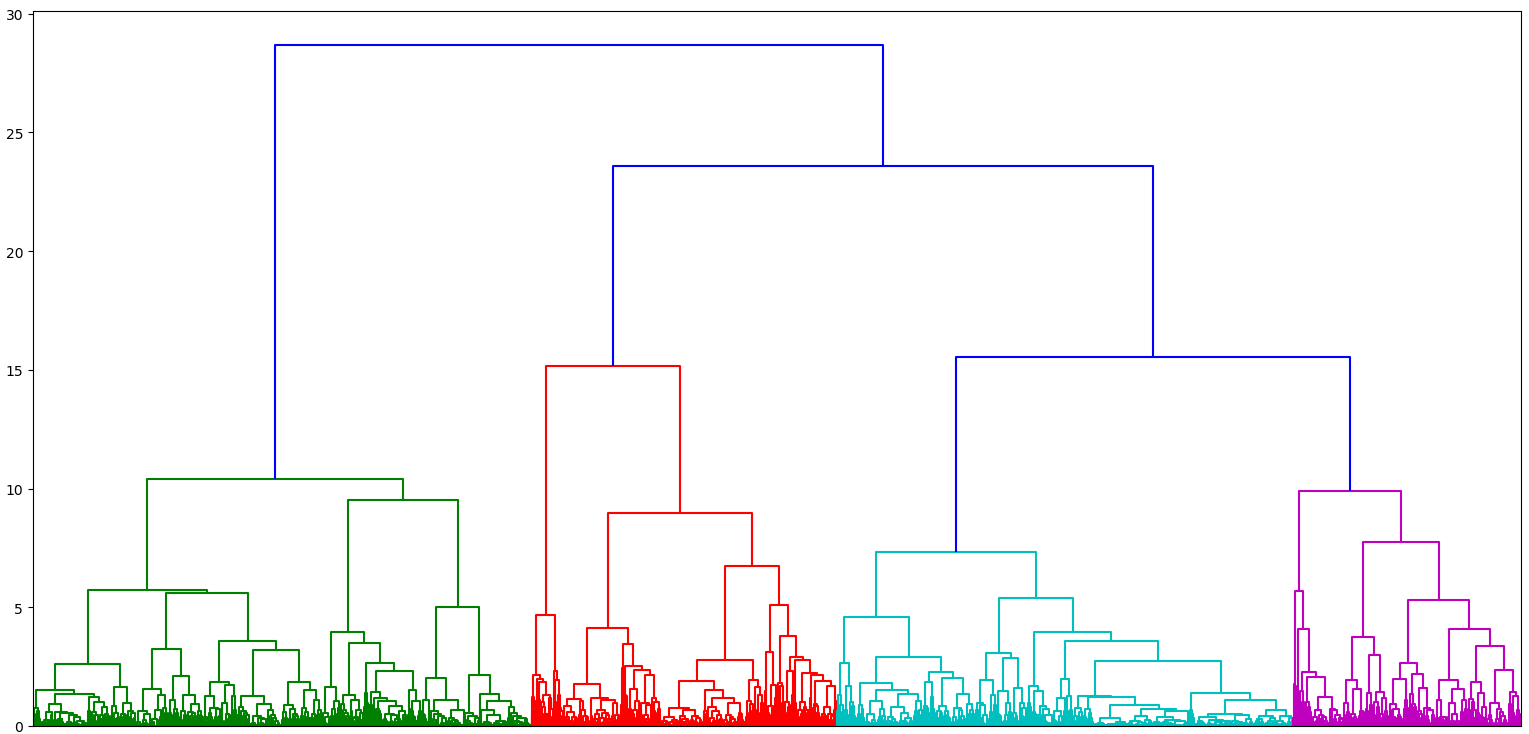
\includegraphics[width=\linewidth]{img/euclidean-ward.png}
  \caption{}\label{euward}
\endminipage\hfill
\minipage{0.48\textwidth}
  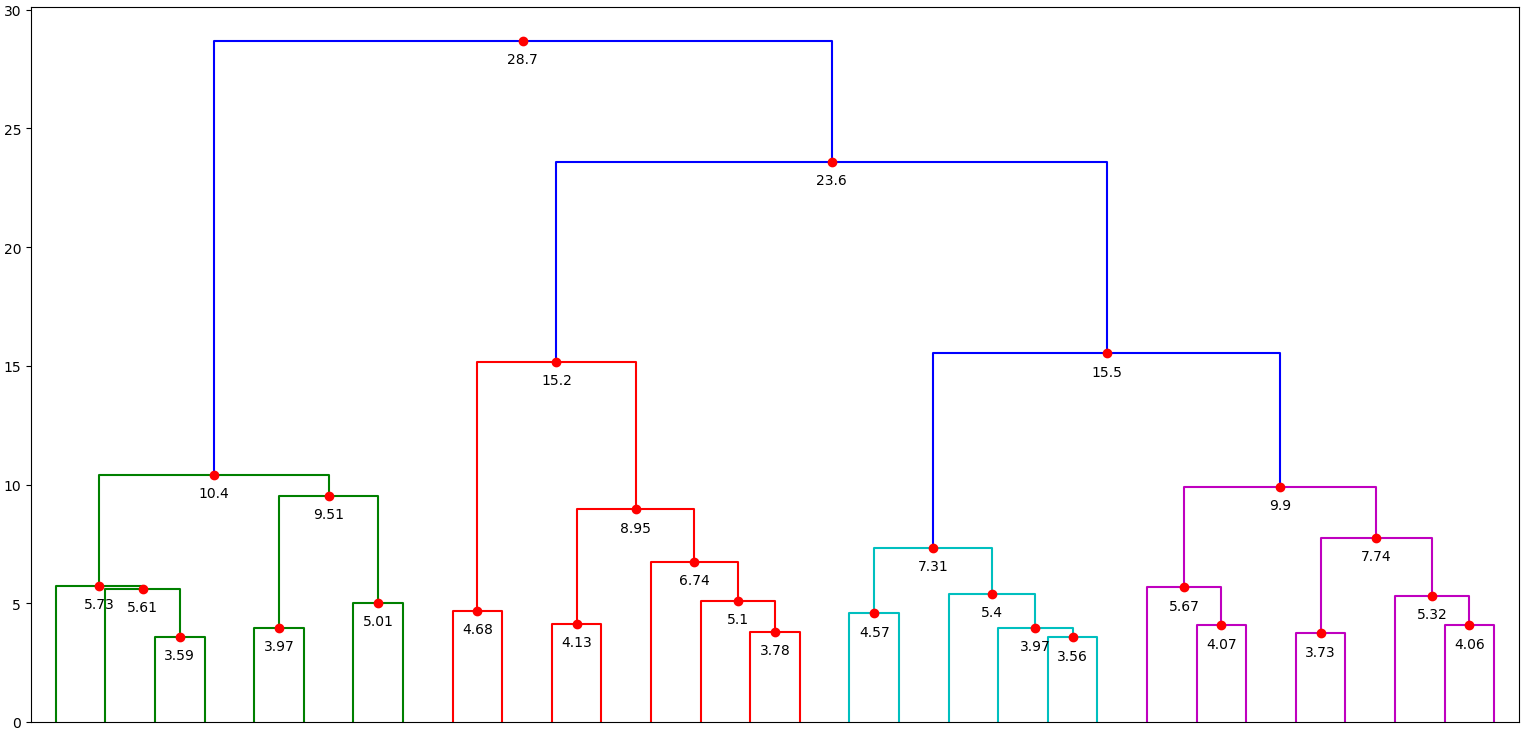
\includegraphics[width=\linewidth]{img/euclidean-ward-truncate.png}
  \caption{}\label{euwardtrunc}
\endminipage\hfill
\end{figure}

\begin{figure}[H]
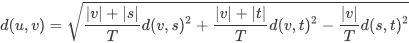
\includegraphics[width=0.5\linewidth]{img/ward_linkage.png}
\centering
\caption{Formula metodo di Ward}
\label{dendro-complete}
\end{figure} 

La Figura 2.7 descrive il metodo di Ward, metodo che cerca di minimizzare la varianza e generare cluster pi\`u coesi possibili. Nella formula $u$ \`e il cluster generato dai cluster $s$ e $t$, $v$ \`e un cluster inutilizzato e $T$ \`e la somma delle cardinalità dei cluster tale che $T = |v| + |s| + |t|$.

I cluster trovati somigliano moltissimo agli stessi cluster trovati di KMeans.
Anche in questo caso infatti, oltre ai cluster dei \textit{senza rischio} e
dei \textit{ritardatari}, abbiamo una divisione sulla base dell'entit\`a delle spese
mensili, formando quindi altri due cluster di \textit{piccoli e grandi pagatori}.
Per la descrizione dei cluster rimandiamo alla descrizione dei cluster di KMeans.

\begin{center}
\begin{tabular}{c|c|c|c|c|c|c}
	\hline
	\textbf{Cluster} & \textbf{ps-sep} 
	& \textbf{ps-aug} & \textbf{pa-sep} 
	& \textbf{pa-aug}\\
	\hline
	Cluster 1 & 
	$ -0.01 (\pm 0.5)$ & 
	$ -0.05 (\pm 0.46)$ &
	$11.8k (\pm 28.1k)$ &
	$14.2k (\pm 44.6)$\\
	\hline
	Cluster 2 & 
	$-0.68 (\pm 1.08)$ & 
	$-1.18 (\pm 0.72)$ &
	$4.8k (\pm 11.6k)$ &
	$4.8k (\pm 13.2k)$\\
	\hline
	Cluster 3 & 
	$1.7 (\pm 0.99)$ & 
	$1.8 (\pm 0.94)$ &
	$1.8k (\pm 3.3k)$ &
	$2.4k (\pm 3.9k)$\\
	\hline
	Cluster 4 & 
	$-0.10 (\pm 0.48)$ & 
	$-0.02 (\pm 0.56)$ &
	$4.2k (\pm 9.9k)$ &
	$3.4k (\pm 8.0k)$\\
	\hline
	& 
	\textbf{ba-sep} & 
	\textbf{ba-aug} & 
	\textbf{limit} & 
	\textbf{age} &\\
	\hline
	Cluster 1 & 
	$152k (\pm 97k)$ &
	$145k (\pm 94k)$ &
	$246k (\pm 126k)$ &
	$36 (\pm 8)$\\
	\hline
	Cluster 2 &
	$10.5k (\pm 21.8k)$ &
	$9k (\pm 19k)$ &
	$214.3k (\pm 125.3k)$ &
	$36 (\pm 8)$\\
	\hline
	Cluster 3 &
	$48.9k (\pm 49k)$ &
	$48k (\pm 48.1k)$ &
	$85.8k (\pm 71.7k)$ &
	$34 (\pm 9)$\\
	\hline
	Cluster 4 &
	$30.2k (\pm 24.3k)$ &
	$29.4k (\pm 22.7k)$ &
	$103.4k (\pm 85.4k)$ &
	$34 (\pm 9)$\\
	\hline
	& 
	\textbf{sex} & 
	\textbf{status} & 
	\textbf{education} & 
	\textbf{default}\\
	\hline
	Cluster 1 & 
	F &
	Single &
	University&
	12\%\\
	\hline
	Cluster 2 & 
	F &
	Single &
	Graduate School&
	15\%\\
	\hline
	Cluster 3 & 
	F &
	Single &
	University&
	60\%\\
	\hline
	Cluster 4 & 
	F &
	Single &
	University&
	16\%\\
	\hline
\end{tabular}
\end{center}

\section{Analisi del miglior clustering e precisazioni}
Prima di passare alle analisi del miglior clustering ottenuto, teniamo
a specificare che DBSCAN \'e stato eseguito su un dataset modificato
ad hoc per il suo funzionamento. Questo stesso dataset, composto da soli
\texttt{payment status} che a nostro avviso \'e l'attributo con pi\`u
carico semantico a disposizione per la nostra analisi, \'e stato usato
successivamente anche con KMeans e Hierarchical. Rieseguendo tutto, essi
con un taglio a quattro cluster suddividevano in modo anomalo il cluster dei
\textit{ritardatari} in base alla gravit\`a dei ritardi stessi.
Con tre cluster entrambi suddividevano il dataset in \textit{senza rischio},
\textit{ritardatari} e persone che utilizzavano intensivamente il revolving credit.
Sebbene l'indice di \sil sia molto pi\`u alto, abbiamo preferito tenere per questi due
il clustering sul dataset descritto precedentemente, poich\`e andava a suddividere in
modo pi\`u specifico come il revolving credit veniva utilizzato, in modo da avere 
pi\`u informazioni su chi poteva essere a rischio default. In ogni caso,
la scelta dipende dalla granularit\`a a cui si vuole vedere il clustering.

Detto ci\`o analizzando DBSCAN notiamo che sullo stesso dataset esso differisce
dal fatto che riesce ad individuare un cluster dei \textit{no consumption}.

In conclusione, non pensiamo ci sia un algoritmo che funziona decisamente meglio
degli altri. Tutto dipende da che \textit{cosa} si vuole trovare. 
Ad esempio, se vogliamo fare un'analisi per trovare il modo di
fare spendere di pi\`u ai nostri utenti, allora prenderemo in considerazione
DBSCAN poich\`e abbiamo un cluster di persone che non utilizzano la carta ben
separato dagli altri, il che rende possibile uno studio pi\`u specifico su queste
persone. Se invece si vuole semplicemente evidenziare i clienti pi\`u a rischio qualsiasi
delle tecniche riesce a ben evidenziare il comportamento.

